\documentclass[11pt]{article}
\usepackage[utf8]{inputenc}
\usepackage[T1]{fontenc}
\usepackage{lmodern}
\usepackage[margin=1in]{geometry}
\usepackage{booktabs}
\usepackage{graphicx}
\usepackage{amsmath,amssymb}
\usepackage{xcolor}
\usepackage[numbers,sort&compress]{natbib}
\usepackage[colorlinks=true,linkcolor=black,citecolor=blue,urlcolor=blue]{hyperref}
\usepackage{caption}
\captionsetup{font=small,labelfont=bf}

\title{\textbf{FamBench: Protein--Ligand Affinity Models Are Inflated by\\
Protein-Family Redundancy}}
\author{Mehdi Yazdani Jahromi\\[2pt]\small \texttt{myjahromi@gmail.com}}
\date{\today}

\begin{document}
\maketitle

\begin{abstract}
\noindent
Co-folding models such as Boltz-2 and Nesso-1 report protein--ligand binding-affinity
correlations of Pearson $\approx 0.6$ and are increasingly proposed as fast surrogates for
free-energy perturbation. We show that this headline accuracy is largely an artifact of
\emph{protein-family redundancy} in the test set. Stratifying $3{,}289$ PDBbind complexes by
protein-family size (MMseqs2 30\% clusters), we find that both models' accuracy scales
monotonically with how heavily the family is represented in the PDB: from Pearson
$\approx 0.10$ on singleton families to $\approx 0.55$--$0.59$ on families with $>300$
homologs. A leakage-slope regression (absolute error vs.\ $\log_{10}$ family size, controlling
for the affinity regime) is significantly negative for both co-folders
($t=-7.5$ and $-4.3$) but \emph{flat} for a random-forest QSAR model and a ligand-$k$NN
baseline evaluated under family-disjoint cross-validation. On novel families the ranking
inverts: a shallow, family-disjoint random forest ($r=0.41$) outperforms both
billion-parameter co-folders ($r=0.32$, $0.31$). On a genuinely novel, post-cutoff target
(OpenBind EV-A71 2A protease), neither co-folder reliably beats a molecular-weight baseline
($\rho=0.49$ for Nesso-1, $0.40$ for Boltz-2, vs.\ $0.47$ for molecular weight). We release
\textbf{FamBench}, a plug-in benchmark and Hugging Face dataset that measures affinity
accuracy \emph{as a function of protein-family novelty} rather than as a single correlation,
so that models are judged on the case that matters for a new drug program: a target they have
not seen.
\end{abstract}

\section{Introduction}

Predicting protein--ligand binding affinity from structure is a central problem in
computational drug discovery. A recent wave of \emph{co-folding} models---AlphaFold3
\citep{abramson2024alphafold3}, Boltz-1/2 \citep{wohlwend2024boltz1,passaro2025boltz2},
Chai-1 \citep{chai2024chai1}, and coarse-grained successors such as Nesso-1
\citep{valencelabs2026nesso1} and TerraBind \citep{terray2026terrabind}---predict the bound
complex and, increasingly, the affinity directly. Boltz-2 reports correlations approaching
free-energy perturbation (FEP) at a fraction of the cost \citep{passaro2025boltz2}, and these
numbers are driving adoption in hit identification and lead optimization.

Such models are almost always summarized by a \emph{single} correlation between predicted and
measured affinity on a held-out set. But a single number cannot distinguish a model that has
learned the physics of binding from one that recognizes protein families it saw many times in
the Protein Data Bank (PDB). The distinction is not academic: a medicinal chemistry program
succeeds or fails on \emph{novel} targets, precisely those least represented in public
structural data.

A large literature has documented that ligand-based and docking benchmarks reward memorization
\citep{wallach2018memorization,chen2019dude}, that affinity networks trained on PDBbind rely on
train--test similarity rather than interaction physics
\citep{volkov2022frustration,kanakala2023latentbiases}, and that re-splitting the data to
remove leakage lowers apparent accuracy \citep{li2023leakproof}. What is missing is a
\emph{quantitative, model-agnostic account} of how co-folding affinity accuracy depends on the
one axis that matters most for prospective use---\emph{protein-family novelty}---and a
benchmark that measures it directly.

We make three contributions.
\begin{enumerate}\itemsep2pt
  \item \textbf{We show co-folding affinity accuracy is a redundancy artifact.} On a matched
  set of $3{,}289$ PDBbind complexes, Boltz-2 and Nesso-1 accuracy rises monotonically with
  protein-family size, collapsing toward zero on singleton families
  (Sec.~\ref{sec:redundancy}, Fig.~\ref{fig:dose}).
  \item \textbf{We isolate the mechanism with controls.} A random-forest QSAR model and a
  ligand-$k$NN baseline, evaluated under \emph{family-disjoint} cross-validation, show no such
  gradient; on novel families they \emph{outperform} the co-folders (Sec.~\ref{sec:controls}).
  On a genuinely novel post-cutoff target, neither co-folder beats molecular weight
  (Sec.~\ref{sec:temporal}).
  \item \textbf{We release FamBench}, a plug-in Python/CLI benchmark and Hugging Face dataset
  with confound-guarded metrics, so any affinity model can be scored on its family-novelty
  curve in a few lines (Sec.~\ref{sec:artifact}).
\end{enumerate}

\section{Related Work}

\paragraph{Co-folding affinity models.}
The AlphaFold2 breakthrough \citep{jumper2021alphafold2} was extended to protein--ligand
complexes by AlphaFold3 \citep{abramson2024alphafold3} and open reimplementations such as
Boltz-1 \citep{wohlwend2024boltz1}, Chai-1 \citep{chai2024chai1}, and RoseTTAFold-All-Atom
\citep{krishna2024rfaa}. A second generation targets affinity directly: Boltz-2
\citep{passaro2025boltz2} is, to our knowledge, the first co-folder to approach FEP accuracy,
and Nesso-1 \citep{valencelabs2026nesso1} and TerraBind \citep{terray2026terrabind} follow with
faster coarse-grained representations. They are evaluated by overall correlation, inviting the
generalization questions that have long dogged scoring functions.

\paragraph{Scoring and QSAR baselines.}
Empirical (AutoDock Vina \citep{trott2010vina}, smina \citep{koes2013smina}) and machine-learned
(RF-Score \citep{ballester2010rfscore}, Gnina \citep{mcnutt2021gnina}, AEV-PLIG
\citep{valsson2025aevplig}) scoring functions established learning affinity from structure.
Nearly all are trained and tested on PDBbind \citep{liu2017pdbbind} and CASF-2016
\citep{su2019casf}, with labels from BindingDB \citep{gilson2016bindingdb} and ChEMBL
\citep{mendez2019chembl}, against the FEP+ reference \citep{wang2015fep}.

\paragraph{Leakage and benchmark critiques.}
Wallach and Heifets \citep{wallach2018memorization} showed most ligand-based benchmarks reward
memorization, and Chen et al.\ \citep{chen2019dude} traced deep-learning ``success'' on DUD-E to
dataset bias. For affinity, Volkov et al.\ \citep{volkov2022frustration} found ligand-only and
protein-only models match full-complex models, and nearest-training-neighbor baselines are
already strong---evidence of memorization. Kanakala et al.\ \citep{kanakala2023latentbiases}
confirmed latent biases in popular sets. The community response has been to re-split:
Leak-Proof PDBBind \citep{li2023leakproof} removes cross-contamination and shows retrained
models generalize better; curated resources such as MISATO \citep{siebenmorgen2024misato} follow
suit.

\paragraph{Time-split and out-of-distribution evaluation.}
Sheridan \citep{sheridan2013timesplit} argued that time-split, not random split, estimates
prospective accuracy. The most stringent test is a target released after a model's training
cutoff; the OpenBind EV-A71 2A protease release \citep{openbind2026dataset} provides exactly such
a post-2021 target, free of PDBbind contamination.

\paragraph{Our contribution.} Prior work establishes that benchmarks reward memorization and
that re-splitting mitigates it. Unlike LP-PDBBind \citep{li2023leakproof}, which fixes a split
and reports one aggregate number, we treat \emph{redundancy as the independent variable} and
expose the accuracy-versus-novelty curve directly, for the newest class of models (co-folders)
that no prior leakage study covers.

\section{The FamBench Benchmark}
\label{sec:artifact}

FamBench comprises two evaluation sets and a set of confound-guarded metrics.

\paragraph{Redundancy set.} $18{,}759$ protein--ligand complexes derived from PDBbind
\citep{liu2017pdbbind} with an exact ($=$) $K_d$, $K_i$, or IC$_{50}$ label converted to
$\mathrm{p}K=-\log_{10}(\text{conc})$. For each complex we record the protein sequence, ligand
SMILES, and---critically---the \emph{protein-family size}: the number of complexes in the same
MMseqs2 \citep{steinegger2017mmseqs2} cluster at 30\% identity / 80\% coverage. Family sizes
range from $1$ (890 singletons) to $809$, over $2{,}203$ families. We define six redundancy
bins ($1$, $2$--$5$, $6$--$20$, $21$--$80$, $81$--$300$, $301+$) and a balanced
``core'' subset of $3{,}360$ complexes (560 per bin) for quick evaluation. A ligand
nearest-neighbor Tanimoto (ECFP4) is also recorded as a secondary novelty axis.

\paragraph{Temporal set.} $649$ compounds with measured $K_d$ against a single, structurally
novel, post-2021 target: the Enterovirus~A71 2A protease from the OpenBind consortium release
\citep{openbind2026dataset} (CC0). Because the target post-dates the 2021-09-30 training cutoff
of the models we evaluate, it is a genuine out-of-distribution test. We ship the consortium's
molecular-weight, clogp, Gnina, smina, AEV-PLIG, and AQ-Affinity predictions as baselines.

\paragraph{Metrics.} The primary quantity is not a single correlation but its dependence on
family size. For each redundancy bin we report Pearson $r$ between predicted and measured
affinity within a \emph{matched} $\mathrm{p}K$ window $[4.5, 8.0]$, which holds the label
spread (and therefore the maximum attainable correlation) approximately constant across bins.
We summarize the whole curve with two headline numbers:
\begin{itemize}\itemsep1pt
  \item \textbf{Novel-family Pearson}: accuracy on families of size $\leq 5$ (the number a model
  should report for a new target).
  \item \textbf{Leakage slope}: the coefficient of $\log_{10}(\text{family size})$ in an ordinary
  least-squares regression of absolute error on family size, the affinity regime ($\mathrm{p}K$,
  $\mathrm{p}K^2$), and affinity type. A significantly negative slope means accuracy is
  \emph{bought by redundancy}.
\end{itemize}
Per-bin confidence intervals are non-parametric bootstrap ($2{,}000$ resamples). On the temporal
set we report within-target Spearman $\rho$ and the residual $\rho$ after linearly removing
molecular weight, which quantifies signal \emph{beyond} ligand size.

\section{Experimental Setup}

We evaluate six methods spanning three families. \textbf{Co-folders:} Boltz-2
\citep{passaro2025boltz2} (with cuEquivariance kernels and ColabFold MSAs) and Nesso-1
\citep{valencelabs2026nesso1} (ESM-2 embeddings \citep{rives2021esm}), both run from public
weights with their default settings; both output $\log_{10}(\text{IC}_{50})$, which we negate to
the FamBench ``higher-is-stronger'' convention. \textbf{Shallow learned baselines:} a
random-forest QSAR model (RF-QSAR) on ECFP4 (1024 bit) plus amino-acid composition, and a
ligand-$k$NN memorization baseline ($k{=}5$, ECFP4 Tanimoto). Both are evaluated under
\emph{5-fold family-disjoint} (\texttt{GroupKFold} on family id) cross-validation, so their
predictions are always on held-out families---the honest counterpart to the co-folders, whose
test families \emph{are} present in their PDB training data. \textbf{Trivial baselines:}
molecular weight and clogp. All methods are scored on the same $3{,}289$-complex intersection
(Boltz-2 on a $578$-complex subset owing to its higher per-target cost).

\section{Results}

\subsection{Co-folding accuracy scales with protein-family redundancy}
\label{sec:redundancy}

Table~\ref{tab:main} reports overall, novel-family, and redundant-family accuracy, together
with the leakage slope. Overall, the co-folders lead (Nesso-1 $r=0.588$), consistent with their
published numbers. But that lead is concentrated on redundant families: Nesso-1 reaches
$r=0.599$ on families with $\geq 81$ homologs and only $r=0.324$ on families of size $\leq 5$.
Boltz-2 shows the same pattern more sharply ($0.429$ vs.\ $0.308$).

\begin{table}[t]
\centering
\small
\caption{Affinity accuracy on the $3{,}289$-complex matched set. Overall and per-stratum Pearson
$r$; the \emph{leakage slope} is the coefficient (with $t$-statistic) of
$\log_{10}(\text{family size})$ in the absolute-error regression. Co-folders have a large,
significant negative slope; family-disjoint and trivial baselines do not. Boltz-2 is scored on a
$578$-complex subset.}
\label{tab:main}
\begin{tabular}{lccccc}
\toprule
Method & Type & Overall $r$ & Novel-fam.\ $r$ & Redund.-fam.\ $r$ & Leakage slope ($t$) \\
\midrule
Nesso-1     & co-folder            & \textbf{0.588} & 0.324 & \textbf{0.599} & $-0.109\ (-7.5)$ \\
Boltz-2     & co-folder            & 0.467 & 0.308 & 0.429 & $-0.139\ (-4.3)$ \\
RF-QSAR     & family-disjoint ML   & 0.479 & \textbf{0.411} & 0.320 & $+0.008\ (+0.6)$ \\
ligand-$k$NN& family-disjoint ML   & 0.407 & 0.350 & 0.374 & $-0.002\ (-0.1)$ \\
clogp       & trivial              & 0.284 & 0.121 & 0.234 & $+0.010\ (+1.0)$ \\
mol.\ weight& trivial              & 0.069 & 0.119 & 0.184 & $+0.017\ (+2.0)$ \\
\bottomrule
\end{tabular}
\end{table}

The matched-$\mathrm{p}K$ dose-response (Table~\ref{tab:dose}, Fig.~\ref{fig:dose}) makes the
effect unambiguous. With label spread held constant across bins, Nesso-1 rises from $r=0.105$ on
singletons to $0.551$ on the largest families; Boltz-2 is statistically \emph{zero} on all
families of size $\leq 20$ ($r=-0.03$ to $-0.01$) and only acquires signal above $21$ homologs.
Because the window pins the attainable correlation, this gradient cannot be explained by
narrower affinity ranges in small families.

\begin{table}[t]
\centering
\small
\caption{Matched-$\mathrm{p}K$ Pearson $r$ by protein-family size. The co-folders rise steeply
with redundancy; the family-disjoint baselines are flat. ($n\approx 350$ per Nesso-1 bin.)}
\label{tab:dose}
\begin{tabular}{lcccccc}
\toprule
Method & \multicolumn{6}{c}{protein-family size} \\
\cmidrule(lr){2-7}
 & 1 & 2--5 & 6--20 & 21--80 & 81--300 & 301+ \\
\midrule
Nesso-1      & 0.105 & 0.225 & 0.378 & 0.421 & 0.437 & \textbf{0.551} \\
Boltz-2      & $-0.030$ & $-0.007$ & $-0.008$ & 0.420 & 0.371 & \textbf{0.585} \\
RF-QSAR      & 0.259 & 0.264 & 0.257 & 0.254 & 0.196 & 0.177 \\
ligand-$k$NN & 0.215 & 0.223 & 0.192 & 0.236 & 0.174 & 0.180 \\
mol.\ weight & $-0.032$ & 0.009 & $-0.101$ & 0.107 & 0.070 & $-0.010$ \\
\bottomrule
\end{tabular}
\end{table}

\begin{figure}[t]
\centering
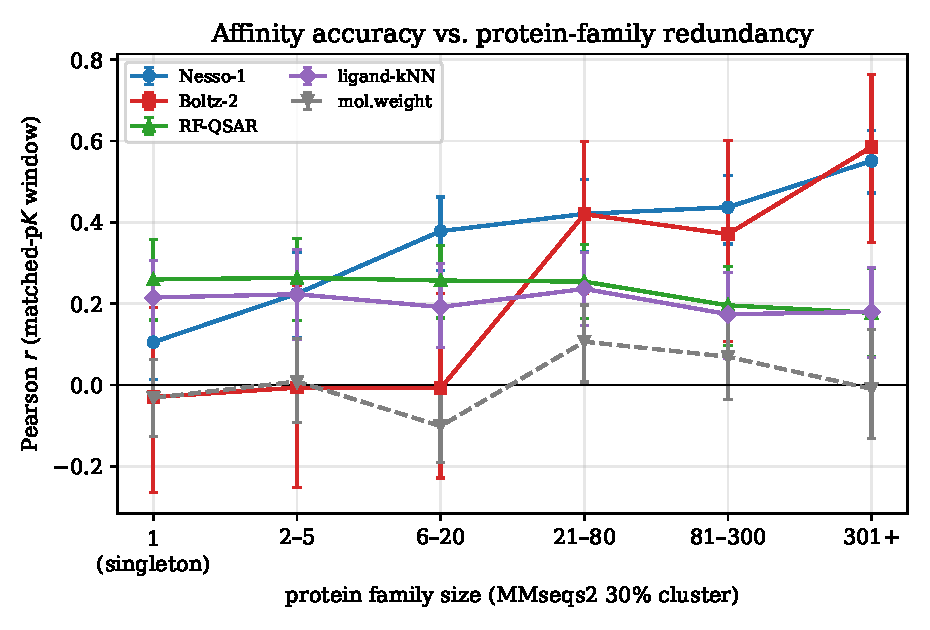
\includegraphics[width=0.68\linewidth]{figures/fig1_dose_response.pdf}
\caption{Affinity accuracy versus protein-family redundancy (matched-$\mathrm{p}K$ window,
bootstrap 95\% CIs). Co-folders (Nesso-1, Boltz-2) rise steeply with family size; a
family-disjoint random forest and ligand-$k$NN are flat. The co-folders' apparent superiority
is confined to redundant families.}
\label{fig:dose}
\end{figure}

\subsection{Controls isolate leakage as the mechanism}
\label{sec:controls}

The two shallow baselines are the diagnostic. Evaluated under family-disjoint
cross-validation---so they can never have ``seen'' the test family---RF-QSAR and ligand-$k$NN
have leakage slopes indistinguishable from zero ($t=+0.6$ and $-0.1$; Fig.~\ref{fig:slope}) and
flat dose-response curves (Table~\ref{tab:dose}). The gradient is therefore not an intrinsic
property of ``harder'' novel targets (which would penalize every method equally); it appears
\emph{only} for models whose training data contains the test families. When family leakage is
removed by construction, the gradient vanishes.

The practical consequence is a rank inversion (Fig.~\ref{fig:novel}). On novel families
(size $\leq 5$), the family-disjoint random forest ($r=0.411$) \emph{outperforms} both
co-folders (Nesso-1 $0.324$, Boltz-2 $0.308$), and even ligand-$k$NN ($0.350$) is competitive. A
model with $10^3$ parameters and no structure beats billion-parameter co-folders on exactly the
regime that matters for a new target.

\begin{figure}[t]
\centering
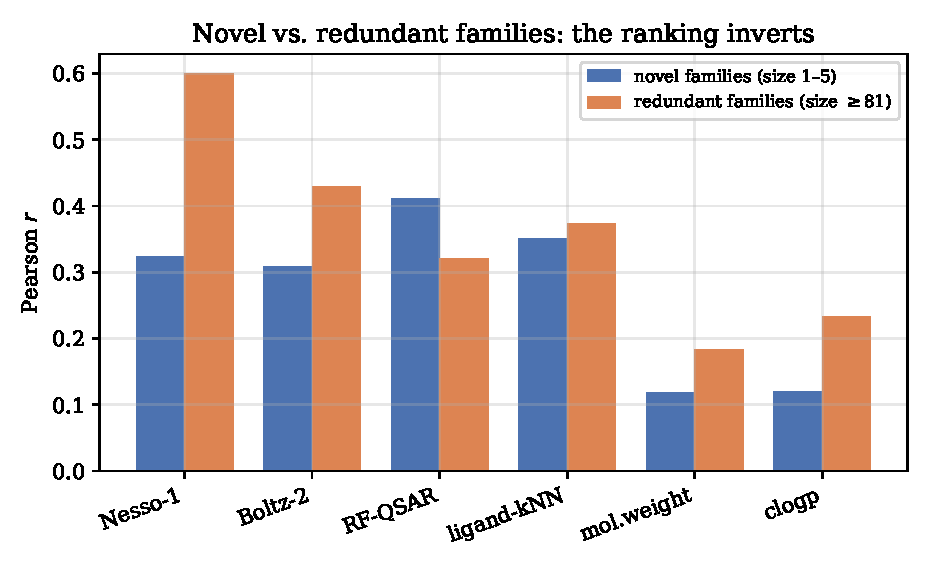
\includegraphics[width=0.49\linewidth]{figures/fig2_novel_vs_redundant.pdf}\hfill
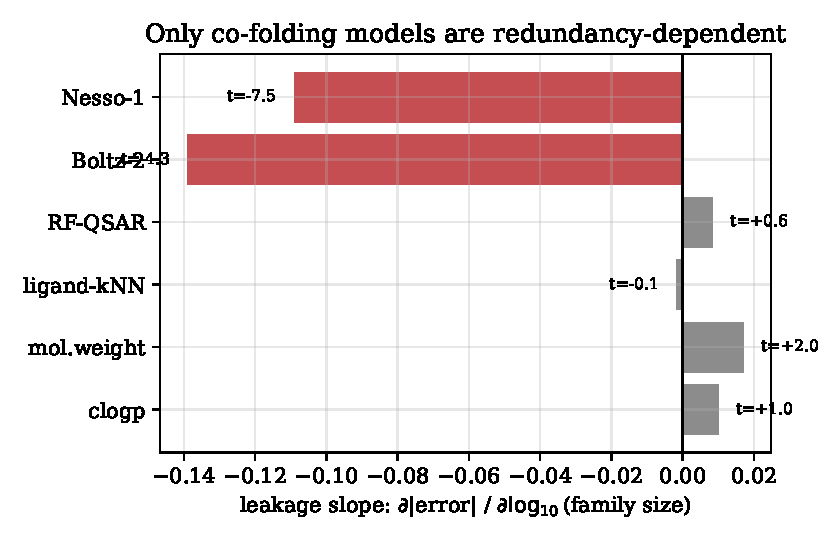
\includegraphics[width=0.49\linewidth]{figures/fig3_leakage_slope.pdf}
\caption{\textbf{Left:} novel- vs.\ redundant-family Pearson $r$. The co-folders' advantage is
entirely on redundant families; on novel families the ranking inverts. \textbf{Right:} leakage
slope (change in $|$error$|$ per decade of family size). Only the co-folders are significantly
redundancy-dependent ($|t|>2$, red).}
\label{fig:slope}
\label{fig:novel}
\end{figure}

\subsection{On a novel target, co-folders do not beat molecular weight}
\label{sec:temporal}

The temporal set removes any ambiguity about ``family size'' as a proxy: the EV-A71 2A protease
post-dates the models' training cutoff and shares no family with PDBbind at the evaluation
threshold. Table~\ref{tab:temporal} reports within-target Spearman $\rho$ over $643$ compounds.
Molecular weight alone achieves $\rho=0.469$. Nesso-1 barely exceeds it ($0.486$); Boltz-2
\emph{underperforms} it ($0.395$), as do Gnina, smina, AEV-PLIG, AQ-Affinity, and clogp. After
residualizing on molecular weight, Nesso-1 retains a modest $\rho=0.233$ of genuine signal and
Boltz-2 only $0.112$; the docking and other ML scorers retain essentially none. On a target no
model has seen, sophisticated affinity prediction collapses to ligand size.

\begin{table}[t]
\centering
\small
\caption{Novel-target ranking (OpenBind EV-A71 2A protease, $643$ compounds). Spearman $\rho$
with experiment, and $\rho$ after removing molecular weight. No method reliably beats the
molecular-weight baseline.}
\label{tab:temporal}
\begin{tabular}{lcc}
\toprule
Method & Spearman $\rho$ & $\rho$ beyond mol.\ weight \\
\midrule
Nesso-1            & \textbf{0.486} & 0.233 \\
molecular weight   & 0.469 & --- \\
Gnina              & 0.431 & $-0.082$ \\
Boltz-2            & 0.395 & 0.112 \\
smina              & 0.229 & $-0.009$ \\
AEV-PLIG           & 0.228 & $-0.143$ \\
clogp              & 0.163 & $-0.057$ \\
AQ-Affinity        & 0.134 & $-0.019$ \\
\bottomrule
\end{tabular}
\end{table}

\begin{figure}[t]
\centering
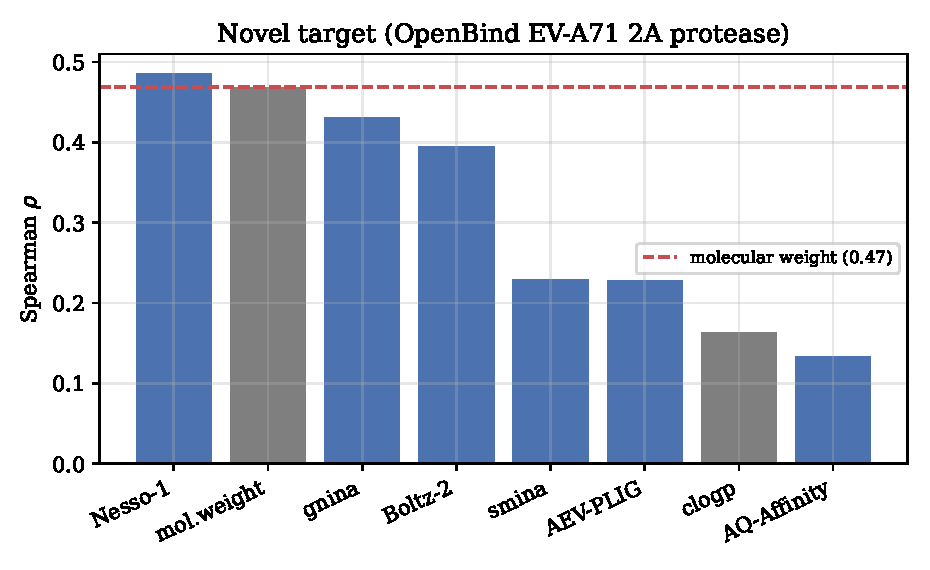
\includegraphics[width=0.62\linewidth]{figures/fig4_temporal.pdf}
\caption{Within-target Spearman $\rho$ on the novel OpenBind target. The dashed line is the
molecular-weight baseline; only Nesso-1 marginally exceeds it.}
\label{fig:temporal}
\end{figure}

\section{Discussion}

Three findings cohere into a single message. First, co-folding affinity accuracy is a
\emph{monotone function of protein-family redundancy}, not a fixed property of the model.
Second, the effect is specifically \emph{leakage}: matched controls that cannot memorize the
family show no gradient, and on novel families they win. Third, the endpoint of the
gradient---a genuinely novel target---is a regime where the state of the art does not beat
molecular weight.

This does not imply co-folders are useless; on well-populated families they are the most
accurate methods we tested. It implies that the standard practice of reporting a single overall
correlation \emph{systematically overstates prospective accuracy}, because public test sets are
dominated by redundant families. A reader who sees ``Pearson $0.6$'' should ask ``on which
families?''---the honest number for a new target is closer to $0.1$--$0.3$. Our controls also
suggest a cheap, strong prospective baseline that is rarely reported: a family-disjoint QSAR
model.

\paragraph{Limitations.} The redundancy set is derived from PDBbind and is therefore
pre-cutoff; its leakage is redundancy-based, and we use family size as a proxy for training
representation. The temporal set removes this proxy but is a single target with a congeneric
compound series, so its absolute numbers should not be over-generalized. We evaluate public
weights at default settings and do not retrain the co-folders on de-leaked data; whether
retraining closes the gap (as for classical scorers \citep{li2023leakproof}) is open. Finally,
family size at 30\% identity is one redundancy axis; ligand-scaffold redundancy is a
complementary axis we record but do not analyze here.

\section{Reproducibility and Artifact}

FamBench is released as an installable package (\texttt{pip install fambench}) with a Hugging
Face dataset. Scoring a model requires wrapping it as
\texttt{predict(sequence, smiles)\,$\to$\,float} and calling \texttt{run\_redundancy} and
\texttt{run\_temporal}; a language-agnostic CLI (\texttt{fambench score}) scores a predictions
CSV. All metrics, confound guards (matched-$\mathrm{p}K$ windows, leakage-slope regression,
bootstrap CIs), baselines, and the dataset-construction pipeline are included. Every number in
this paper is reproduced by the shipped harness from the released predictions.

\section{Conclusion}

Binding-affinity leaderboards for co-folding models measure the wrong thing: accuracy on
protein families the model has already seen. FamBench re-centers evaluation on
protein-family novelty, exposes a steep redundancy gradient in Boltz-2 and Nesso-1, and shows
that on a novel target neither beats molecular weight. We hope reporting the novel-family
number and the leakage slope---rather than a single correlation---becomes standard practice for
the next generation of affinity models.

\paragraph{Data and code availability.}
Benchmark, code, and figures: \url{https://github.com/mrnafold/fambench}.
Dataset: \url{https://huggingface.co/datasets/mrnafold/fambench}.

{\small
\bibliographystyle{unsrtnat}
\bibliography{references}
}

\end{document}
